\documentclass{fhnwreport}
\usepackage[ngerman]{babel}
\usepackage[T1]{fontenc}
\usepackage[latin1]{inputenc}
\usepackage{tikz}
\usepackage{amsmath}
\usetikzlibrary{arrows}
\usepackage{lmodern}
\usepackage[final]{pdfpages}
\usepackage{graphicx}

\title{%
  \textsc{Projekt 2}\\[2ex]
  \textsc{Statusbericht 1}}
\author{%
  \textsc{Team1}}
\date{%
  \textsc{01.04.2015}}

%\textit{} % italics
%\textbf{} % bold
%\texttt{} % typewriter style
%\textsf{} % sans-serif
%\textsc{} % all capital letters

\begin{document}
\maketitle

\vfill

\textsc{%
\begin{tabbing}
Auftraggeber: \hspace{4em} \=  Peter Niklaus \\[2ex]
Betreuer:  \>  Pascal Buchschacher, Anita Gertiser \\[2ex]
Experten:  \>  Peter Niklaus, Richard Gut \\[2ex]
Team:  \> Alexander Stocker \\ 
\> Claudius J�rg \\
\> Denis Stampfli \\
\> Martin Moser \\
\> Reto Freivogel \\
\> Yohannes Measho \\ [2ex]
Studiengang: \> Elektro- und Informationstechnik
\end{tabbing}}

\clearpage

\tableofcontents
\newpage

\section{Projektstatus, Zusammenfassung}
\subsection{Highlights}
\begin{itemize}
	\item Bereits nach kurzer Zeit hat sich unser 							Fachspezialist Martin Moser einen genaueren 					�berblick �ber den Ablauf der Phasengangmethode 				gemacht. Seine Erkenntnis hat er in Form eines 					Flussdiagrammes festgehalten.
	\item Unsere Java Gruppe erarbeitete sich in kurzer Zeit 				ein GUI-Entwurf, mit welchem ge/-arbeitet werden 				kann.
\end{itemize}
\subsection{Lowlights}
\begin{itemize}
	\item Uneinigkeiten im Team haben Zeit gekostet.
	\item Unklare Auftragserteilungen brachten ein falsches 				Ergebnis.
\end{itemize}
\subsection{Kritische Punkte}
\begin{itemize}
	\item Zurzeit ist das Layout nur einmal mit Herr Niklaus 				besprochen worden, einen zweiten Termin ist noch 				ausstehend.
\end{itemize}
\subsection{Hauptereignisse der vergangene Periode}
\begin{itemize}
	\item Recherchieren
	\item Pflichtenheft erstellt
	\item Beispiel Rechnungen im Matlab gerechnet
\end{itemize}
\subsection{Bevorstehende Hauptereignisse}
\begin{itemize}
	\item Software erstellen ohne graphische Auswertung
	\item Matlab-Files in Java-Code �bersetzten. 
\end{itemize}

\section{Technischer Status}
\subsection{AP Fortschritt}
Nach der Auftragskl�rung vom Kick-off-Meeting las sich das Team in die verschiedenen Themenbereiche ein. Es entstanden Zusammenfassung, welche das Team w�hrend der Auftragskl�rung unterst�tzt. Der Projektleiter teilte sein Team in drei kleine Arbeitsgruppen ein. Die Arbeitsgruppe Elektrotechnik verschaffte sich in der ersten Phase einen �berblick �ber die Phasengangmethode, die Faustformel und das Matlabfile mit der Sanimethode. W�hrend der Recherche erarbeitete sich die Arbeitsgruppe einen schematischen Ablauf der Berechnung. Relevante Zusammenh�nge der Reglungstechnik und der Phasengangmethode hat die Gruppe in einem Dokument zusammengetragen. Der gr�sste Teil wurde ins Pflichtenheft geschrieben. Das Matlabfile mit der Sanimethode, welches von Prof Niklaus zur Verf�gung gestellt wurde, wurde ausgiebig getestet. Die Fachgruppe versteht die Ausgegeben Werte und kann diese Werte weiterverwenden. Zudem haben sie einige Matlabfiles erstellt, welche den Prozess der Phasengangmethode ersetzt. Die zweite Fachgruppe ?Gruppe-Java? erarbeitete sich w�hrend der ersten Phase einen �berblick �ber die verschiedenen Java-Klassen. Zus�tzlich erstellten sie eine erste Version des Layouts. Die Fachgruppe Java erarbeitete sich ein graphisches Konzept, welches die Anwendungsf�lle enth�lt. 
\subsection{Geplante Aktivit�ten f�r die n�chste Periode}
In der n�chsten Periode nehmen wir die Realisierung der Software in Visier. Prim�r geht es dabei um die �bersetzung der diversen Matlabskripte. Die Skripte sollen so auskommentiert werden, dass unsere Java-Gruppe diese in Java-Code umsetzen k�nnen. Als zweites Ziel und somit auch Folgeziel ist es die Software betriebsf�hig zu machen. Die Software kann am Ender der n�chsten Phase die n�tigen Reglerparameter liefern.

\section{Management Status}
\subsection{Meilensteine und Lieferobjekte Tracking}
\subsubsection{Meilensteine}
\begin{center}
\begin{tabular}{|c|l|p{2cm}|p{2cm}|l|p{3cm}|}
\hline
\textbf{ID} & \textbf{Meilensteine Bezeichnung} & \textbf{Geplantes Datum} & \textbf{Aktuelles Datum} & \textbf{Status} & \textbf{Kommentar}\\
\hline
M1 & Pflichtenheft erstellt & 24.03.15 & 24.03.15 & erreicht & \\
\hline
M2 & Matlabskripte auskommentiert & 15.04.15 &  & In Arbeit & \\
\hline
M3 & Software ohne Graph & 19.04.15 &  & In Arbeit & \\
\hline
M4 & Software mit Graph & 03.05.15 &  & In Arbeit & \\
\hline
M5 & Software mit Optionen und Graph & 08.05.15 &  & In Arbeit & \\
\hline
M6 & Monte-Carlo Analyse & 26.05.15 &  & In Arbeit & \\
\hline
M7 & Abschluss Berichte erstellt & 03.06.15 &  & In Arbeit & \\
\hline
\end{tabular}
\end{center}
\subsubsection{Lieferobjekte}
\begin{center}
\begin{tabular}{|c|l|p{2cm}|p{2cm}|l|p{3cm}|}
\hline
\textbf{ID} & \textbf{Lieferobjekte Bezeichnung} & \textbf{Geplantes Datum} & \textbf{Aktuelles Datum} & \textbf{Status} & \textbf{Kommentar}\\
\hline
D1 & Abgabe Pflichtenheft & 25.03.15 & 25.03.15 & abgegeben & \\
\hline
D2 & Statusbericht 1 & 01.04.15 &  & verz�gert & Durch die Korrektur des Pflichtenhefts verz�gert sich der Statusbericht, da teils Informationen in den Bericht einfliessen.\\
\hline
D3 & Zwischenpr�sentation & 15.04.15 &  & In Arbeit & \\
\hline
D4 & Statusbericht 2 & 29.04.15 &  & In Arbeit & \\
\hline
D5 & Einleitung und Disposition & 29.04.15 &  & In Arbeit & \\
\hline
D6 & Statusbericht 3 & 13.05.15 &  & In Arbeit & \\
\hline
D7 & Statusbericht 4 & 03.06.15 &  & In Arbeit & \\
\hline
D8 & Schlusspr�sentation & 10.06.15 &  & In Arbeit & \\
\hline
D9 & Fachbericht und PMA-Bericht & 10.06.15 &  & In Arbeit & \\
\hline
\end{tabular}
\end{center}
\subsection{Kostentracking}
\subsubsection{Personalkosten}
Abbildung \ref{perskost} zeigt die geplanten (breite S�ule) und die bisher entstandenen (schmale S�ule) Personalkosten (TCHF).
\begin{center}
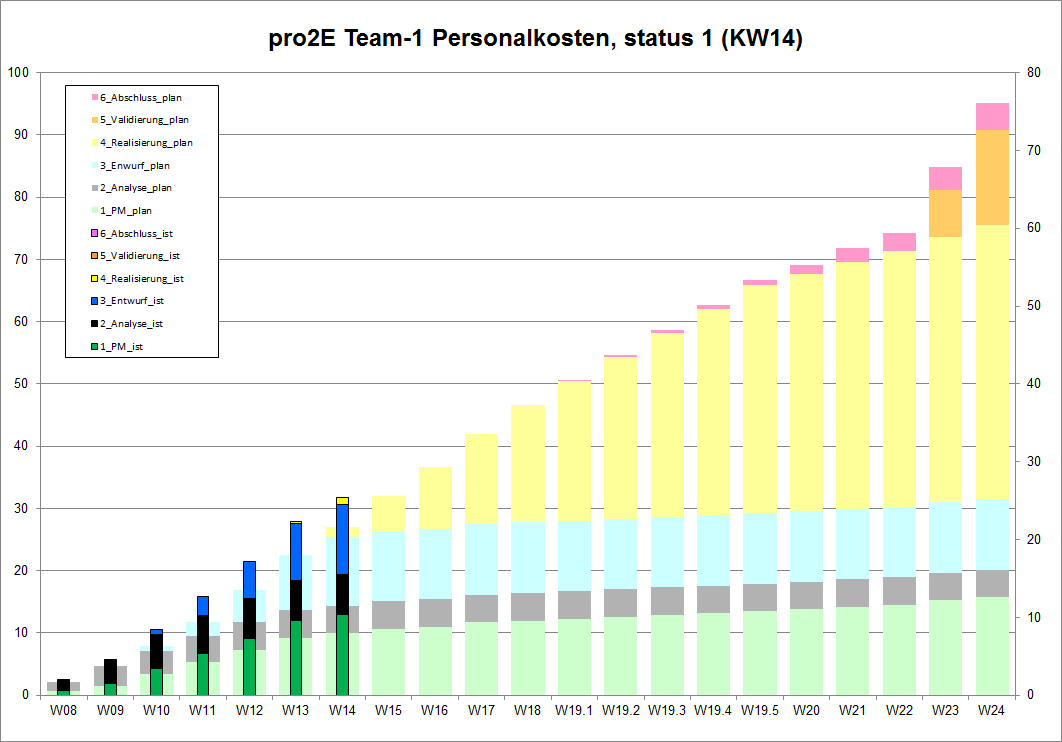
\includegraphics[scale=0.5]{Diagram_stat1}
\end{center}
%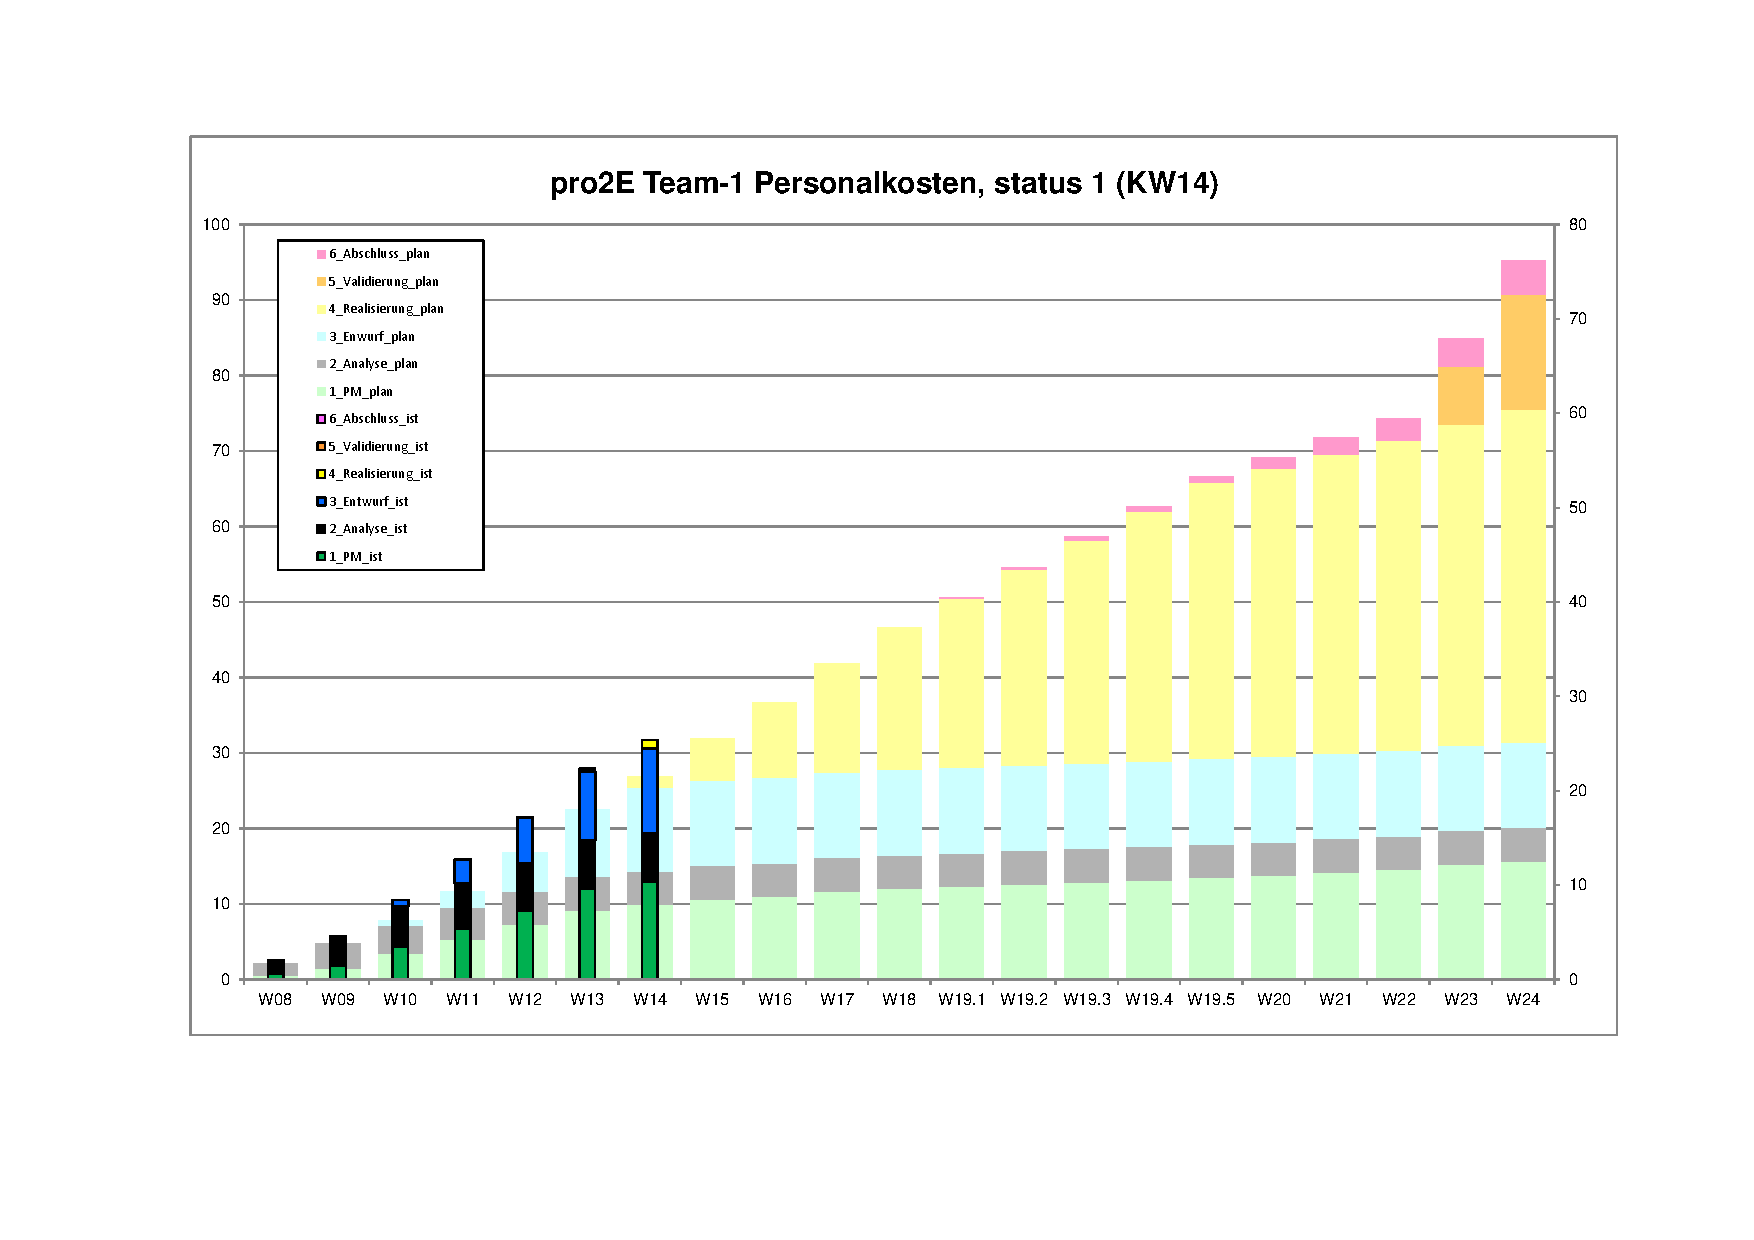
\includepdf[pages=1]{perskostenbalkendiagramm}
Abb. 3.2.1 \label{perskost} Personalkosten Status (Plan / Ist Vergleich)

\subsection{Risiko Tracking}
\subsubsection{Risikoregister Status}
\begin{center}
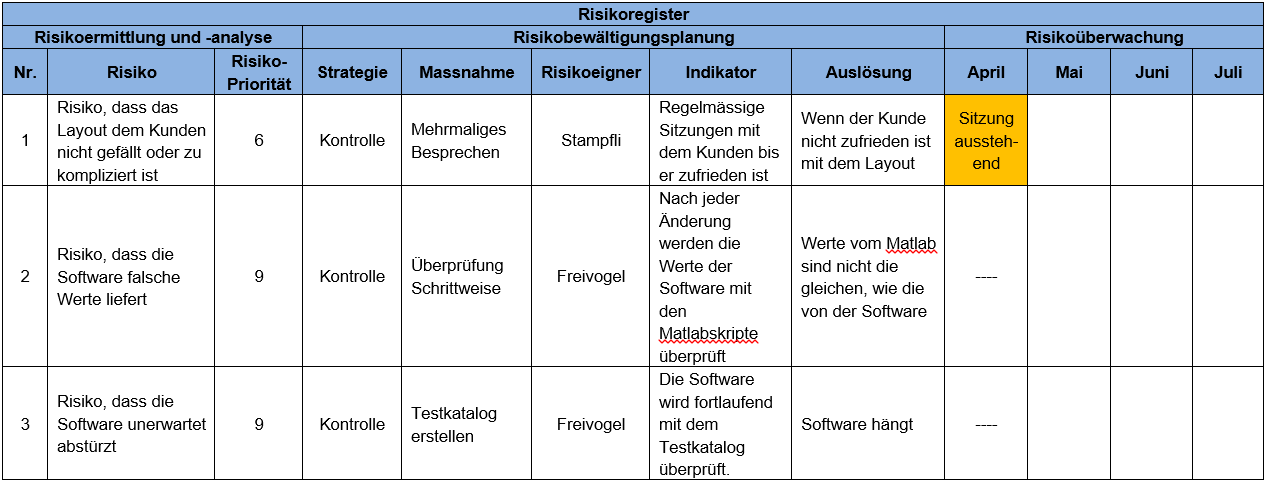
\includegraphics[scale=0.5]{risikoreg_stat1}
\end{center}

\subsubsection{Kommentare}
Auf der technischen Ebene sind bislang keine unvorhergesehenen Risiken eingetroffen. Jedoch ist eine Diskussion im Team entbrannt �ber den Kommunikationsfluss in den Gruppen, unter den Gruppen und zum Teamleiter. Es wurde die Massnahme getroffen, dass Ereignisse ab sofort und von jedem mitgeteilt werden. So dass jedes Mitglied jederzeit �ber die Fortschritte informiert ist.

\end{document}

